\chapter{\Acl{amc}}
\label{chp:amc}
\section{Introduction}
\label{sec:amc-intro}


Link adaptation is a key enabling technology for broadband mobile internet, and has been part of the \gls{5g} \gls{nr} access technology.
%
In this context, \gls{amc} refers to the selection of the appropriate \gls{mcs} as a function of the channel quality, in order to keep the \gls{bler} below a predefined threshold.
%
In 4G long term evolution (LTE), the \gls{bler} target is fixed at 10\% \cite{3gpp.36.213}. However, 5G systems will cover a wider spectrum of services, requiring potentially different \gls{bler} targets \cite{Amin_2016,fantacci2009adaptive}.

%
% \Gls{5g} wireless communication systems are being designed to provide high data and transmission rates \cite{Amin_2016}.
% %
% Because of this, a reliable link adaptation process for \gls{5g} \gls{nr} is needed for coping with the need of increasing the data rate that can be accurately transmitted \cite{chu01}.
% %
%
% In this context, the link adaptation technique of \gls{amc} is of great interest.
% %
% \Gls{amc} is a resource allocation technique used in link adaptation that allows the system to select the most appropriate \gls{mcs} to better cope with the changing channel conditions \cite{fantacci2009adaptive}.
% %

\Gls{amc} is a good solution to match the link throughput to the time-varying nature of the wireless channel under mobility.
%
Periodically, the \gls{ue} measures the channel quality and maps this information into a \gls{cqi}.
%
The \gls{bs} uses the \gls{cqi} reported by the \gls{ue} to define the \gls{mcs}.
%
Typically, each \gls{cqi} is associated with a given \gls{snr} interval \cite{Blanquez-Casado2016}.
%
Considering \gls{lte} as an example, the \gls{bs} uses \gls{dci} embedded into the \gls{pdcch} to inform the \gls{ue} about each new \gls{mcs} selection \cite{ErikDahlman5G}.

%
% In the downlink \gls{amc} procedure, the \gls{ue} suggests to the \gls{bs} an appropriate \gls{mcs} in the \gls{amc} set to be used \cite{Sang2014}.
% %
% This proposed \gls{mcs} is informed to the \gls{bs} by means of a \gls{cqi}, typically each \gls{cqi} represents a \gls{snr} interval \cite{Blanquez-Casado2016}.
% %
% In possession of this information, the \gls{bs} selects an \gls{mcs} to transmit and reports  its selection to the \gls{ue}.

Conventional solutions to the \gls{amc} problem includes the fixed look-up table \cite{fantacci2009adaptive}, also called \gls{illa}, and the \gls{olla} technique, which further improves the look-up table by adapting the \gls{snr} thresholds.
%
The \gls{olla} technique was first proposed in \cite{Sampath1997}, and was also addressed in \cite{Pedersen2007,Sarret2015, Blanquez-Casado2016}.

\Gls{ml} has become an attractive tool to devise novel \gls{amc} solutions in the context of complex emerging \gls{5g} systems and services.
%
In particular the drive towards self-organizing networks is potentially addressed by machine learning.
%
While in \gls{lte}, a look-up table provides fixed \gls{amc} rules for all the users, the emerging systems need a more flexible approach that can automatically adjust physical layer parameters (such as the modulation and coding scheme) according to the user channel state and service type.
%
\Gls{rl} refers to a category of \gls{ml} techniques \cite{survey-son} that has been applied to problems such as backhaul optimization~\cite{jaber2015}, coverage and capacity optimization~\cite{Fan2014} and resource optimization~\cite{Miozzo2017SwitchOnOffPF}.
% The goal of the \gls{amc} is an automatic choice of the best parameters, in this case the \gls{mcs}, depending on the user and applications requirements.
% %
% As such, \gls{ml} algorithms are well suited to this application, because of their capabilities of learning patterns, forecasting behaviors and generating models \cite{survey-son}.
%
% A \gls{ml} category of particular interest to cellular systems is the \gls{rl}, because of its applicability in optimization problems \cite{survey-son}, such as backhaul optimization~\cite{jaber2015}, coverage and capacity optimization~\cite{Fan2014} and resource optimization~\cite{Miozzo2017SwitchOnOffPF}.
There are few works that use \gls{rl} to solve the \gls{amc} problem.
%
In \cite{continuousState}, the selection of the \gls{mcs} is based on the received \gls{sinr}.
%
In this case, the state space is continuous, and the learning algorithm must handle a large state space.
%
In \cite{bruno2014robust} a Q-learning algorithm is proposed to solve the \gls{amc} problem in the context of a 4G \gls{lte} network.
%
A deep reinforcement learning approach is adopted in \cite{DRL_AMC} in the context of a cognitive heterogeneous network.
%


This work proposes a novel 5G \gls{amc} solution based on a \gls{rl} framework.
%
The proposed solution consists of collecting channel measurements at specific time instants to train an agent using the Q-learning algorithm.
%
The trained agent selects  a \gls{mcs} according to SNR measurements to maximize the current spectral efficiency.
%
We assume  a beam-based \gls{5g}-\gls{nr} as access technology, where the transmit and receive beams are selected using the beam sweeping procedure from \cite{giordani21}. The proposed \gls{amc} acts between any two consecutive points of sweeping.
%
We consider that the \gls{snr} between two consecutive points of sweeping tends to decrease due to the \ue~mobility  since it causes a mismatch among beams and the channel paths.
%
The agent uses the trained Q-table and the current measured \gls{snr} to properly select a \gls{mcs}.
%
To the best of authors' knowledge, previous works in \gls{amc} do not address the mismatch among beams and channel paths, while our solution works within the 5G-NR framework.
%%%%%%%%%%%%%%%%%%%%%%%%%%%%%%%%%%--End Of Section--%%%%%%%%%%%%%%%%%%%%%%%%%%%%%%%%%%%%%

\section{System Model}
\label{sec:amc-system-model}
%\subsection{Signal Model}

Consider a single cell system whose \gls{bs} is equipped with \gls{not:txAnt} antennas serving one \gls{ue} with \gls{not:rxAnt} antennas. The signaling period, of duration $T_{SS}$ herein referred to as a \emph{frame}, is divided into two time windows, as shown in Figure \ref{fig:amc-system-timing}. The first one contains a set of synchronization signal (SS) blocks with duration $T_{BS}$, where \emph{beam sweeping} is performed. More specifically, during this time window, the search for the best beam pair happens. The second time window is dedicated to data transmission using the selected beam pair. During this period, of duration $T_{D}$, the UE reports periodically the measured CQI to the BS that responds with the selected MCS.
%
%Assume that the user is synchronized with the  \gls{bs}, and they periodically measure their associated \gls{not:nBeams}  beam pairs.
%Assume that the \gls{bs} sends periodically synchronization signal (SS) blocks used by the \gls{ue} to measure a set of beam pairs and then selecting that one with highest \gls{snr}.
%
%The \bs~and \ue~are assumed to apply \gls{not:Wtx} \inSetComplex{\gls{not:txAnt}}{\gls{not:nBeams}} and \gls{not:Wrx} \inSetComplex{\gls{not:rxAnt}}{\gls{not:nBeams}}, respectively.

During the transmission of the SS blocks, the BS measures all possible combinations of transmit and receive beams from the codebooks \gls{not:Wtx} \inSetComplex{\gls{not:txAnt}}{\gls{not:nBeams}} and \gls{not:Wrx} \inSetComplex{\gls{not:rxAnt}}{\gls{not:nBeams}}, respectively,  to select the beam pair with the highest \gls{snr}.
%
The selected beam pair for the $k$-th frame is expressed as
\begin{equation}
\label{eq.:amc-beam-sweeping}
  \{ \bar{\mathbf{w}}_k, \bar{\mathbf{f}}_k \}= \argmax_{\mathbf{w}, \mathbf{f}} \frac{\|\mathbf{w}^H \mathbf{H}_t \mathbf{f}\|}{\sigma ^2},
\end{equation}
%
\noindent where $\mathbf{f}$ and $\mathbf{w}$ are columns of \gls{not:Wtx} and \gls{not:Wrx}, respectively,  $\channel _t $ \inSetComplex{\gls{not:rxAnt}}{\gls{not:txAnt}} is the channel between the \bs~ and the \ue at time $t$. We assume that the channel remains constant during the beam sweeping period $T_{BS}$.
%
The update of $\{ \bar{\mathbf{w}}_k, \bar{\mathbf{f}}_k \}$ depends on the periodicity $T_{SS}$ of the synchronization signal blocks, which can be  \{5, 10, 20 , 40, 80, 160\} (ms) \cite{giordani21}.
%
Therefore, the each beam pair solution remains constant within the time period $T_{SS}$, until the subsequent SS block arrives, when the BS can reevaluate Eq. \eqref{eq.:amc-beam-sweeping}.
%
%This process is illustrated in Figure \ref{fig:system-timing} that shows the measurement window model, where the \gls{mcs} decision points are the points in which the \gls{bs} and the \gls{ue} exchange information to choose the best \gls{mcs}, as explained in Section \ref{subsec:trans}.


%% explanation of figure
\begin{figure}[tb]
\centerline{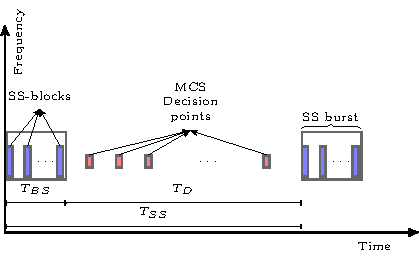
\includegraphics[width=\columnwidth]{figures/chp_amc/amc_q_learning.pdf}}
\caption{Model of time scheduling of operations.}
\label{fig:amc-system-timing}
\end{figure}


During the data transmission window, the discret-time received signal for the $t$-th symbol period associated with the $k$-th fixed beam pair, is given by
\begin{equation}
\label{eq.:amc-rx-signal}
	\gls{not:Y}_{k,t} =
    \bar{\mathbf{w}}^H_k \,
  \channel _t\,
   \bar{\mathbf{f}}_k \,
   \gls{not:sscl}_t
   % _\userIdx
 +
  \bar{\mathbf{w}}^H_k \;
  \gls{not:Z}_t,
\end{equation}

\noindent where $\gls{not:sscl}$ is the symbol transmitted to the \ue, and $\gls{not:Z}_t$ is the additive white Gaussian noise with zero mean and variance \gls{not:var}.
%
%Note that the index $k$ and index $t$ refer to distinct points in time, i.e. the transmit and receive beams can have a mismatch with channel paths depending on \ue~mobility.
%
Defining
\begin{equation}
  \tilde{h}_{k,t} =     \bar{\mathbf{w}}^H_k \,
  \channel _t\,
   \bar{\mathbf{f}}_k \, ,
\end{equation}
as the effective channel at time $t$, associated with the chosen beam pair $\{ \bar{\mathbf{w}}_k, \bar{\mathbf{f}}_k \}$, the effective SNR at the \ue \, is given by
%
\begin{equation}
    \label{eq.:amc-snr}
    \textrm{SNR} = \frac{ \abs{
    % \hermitian{\gls{not:Wrx}\subArg{\userIdx}\argPair{:}{\idxI}}
     \tilde{h}_{k,t}
      % \subArg{\userIdx} \gls{not:Wtx}\subArg{\userIdx}\argPair{:}{\idxJ}
      }^2 }{\gls{not:var}} p_{\gls{not:sscl}},
\end{equation}
%https://www.overleaf.com/project/5d16668cdc29bf0ff4f11132
where $p_{\gls{not:sscl}}$ is the the power of transmitted symbol.
%
%
%\noindent with \gls{not:Wrx}\subArg{\userIdx}\argPair{:}{\idxI} and \gls{not:Wtx}\subArg{\userIdx}\argPair{:}{\idxJ} being the \idxI th and \idxJ th beams of the codebook  \gls{not:Wrx}\subArg{\userIdx} and \gls{not:Wtx}\subArg{\userIdx}, respectively.

% \subsection{Channel Description}
%The model in \eqref{eq.:rx_signal} assumes a narrowband block-fading channel, so the channel is almost constant within a time-frequency resource block \cite{alkhateeb2014}.

%%%%%%%%%%%%%%%%%%%%%%%%%%%%%%%%%%%%%%%%%%%%%%%%%%%%%%%%%%%%%%%%%%%%%%%%%%%%%%%%
